\documentclass[journal,a4paper,twoside]{sty/IEEEtran}

\usepackage[utf8]{inputenc}
\usepackage[slovene]{babel}
\usepackage[T1]{fontenc}
\usepackage{sty/EVrevija}
\usepackage{graphicx}
\usepackage{siunitx}
\usepackage{tikz}
\usepackage{mathtools}
\usepackage{amsmath}
\usepackage[affil-it]{authblk}
\graphicspath{{./Slike/}}
\begin{document}

% naslov prispevka, lahko uporabite en linebreak \\
\title{Regulacija asinhronskega motorja v slabljenju polja}

\authors{Mitja Ali"c} 
\address{E-pošta: mitja1357@gmail.com}

\abstract{
\textbf{IZHODIŠČA}. Potreba po velikem razponu vrtilne hitrosti je v sedanjosti na podro"cju vodenja pogonov zelo potrebna. Z uporabo napetostno-frekven"cnih pretvornikov se lahko generira poljubne oblike in velikosti napajalnih napetosti. Na podlagi razli"cnih tehnik in izra"cunov nastavljamo "zeljene vrednosti za pogone. V tem delu bom predstavil tehnike za regulacijo asinhronskega stroja v podro"cju konstantne mo"ci, pri "cemer je "zelja po "cim vi"sjem ustvarjenem navoru.
\\
\textbf{METODE}. Ob pregledu strokovne literature, ki je ustrezala "studiji, sem zbral primere tehnik, s katerimi asinhronski motor reguliramo v obmo"cju slabljenja polja, hkrati pa zagotovimo visoko vrednost ustvarjenega navora.
\\
\textbf{REZULTATI}. S simulacijami sem prikazal, da s pomo"cjo ra"zli"cnih tehnik, stroj v podro"cju slabljenja polja ustvari razli"cne velikosti elektri"cnega navora.
\\
\textbf{ZAKLJUČEK}. Obstaja veliko pristopov, kako regulirati pogon asinhronskega motorja  v podro"cju slabljenja polja. Razli"cne tehnike se odzivajo razli"cno. S katero tehniko bo motor reguliran, je odvisno le od na"crtovalca pogona.
}

\keywords{koordinatni sistem rotorskega polja, magnetilni tok, navor, slabljenje polja}

% Priimki avtorjev in kratek naslov članka za tekočo glavo
\markboth{Ali"c}{Regulacija asinhronskega motorja v slabljenju polja}

% make the title area
\maketitle

% Naslov in kratek povzetek v angleščini
%\english{Control of asynchronous motor in the field weakening}
%{\textbf{\textit{Abstract:}} {\it \textbf{BACKGROUND}. The need of large range of speed for integrated electric drives is nowadays crucial. Due to AC-AC converters, power signals could have variable amplitude or frequency. An engineer is required to set up the technique for determination of referenced values of currents and voltages.  By using different techniques, electrical drive will respond variously. In this paper I will represent some of the techniques, for setting referenced values of currents in the field weakening range. By using different techniques, torque capability is changed.
%\\
%\textbf{METHODS}.  A systematic search of bibliographic databases was performed. Crucial pieces of information were collected in this document. Few of the techniques has been simulated with Matlab.
%\\
%\textbf{RESULTS}. The results shows, by using different technique for regulation of electrical drive in field weakening range profundly influence on torque capability.
%\\
%\textbf{CONCLUSION}. Setting referenced values of stator currents, dependes of chosen technique. The technique that will be used for electrical drive, it is depending on the constructor.
%}}

\section{Uvod}


"Zelja po velikem razponu vrtilne hitrosti elektromotorjev je v sedanjem "casu zelo za"zeljena. Z uporabo napetostno-frekven"cnih pretvornikov se lahko pogone zelo dobro prilagodi bremenom, katere bo moral premagovati. Z razli"cnimi metodami se pogone lahko vodi v "sirokem obmo"cju. V obmo"cjih do nazivne hitrosti se uporablja metoda U/f \cite{servopogoni}, ki v podro"cju do nazivne hitrosti omogo"ca ustvariti konstanten navor. 
V nadnazivnih hitrostih za"cne pogon omejevati napetostna zmo"znost napajalnega pretvornika.  Navadno se pri tej to"cki obratovanja spremeni metoda za dolo"canje "zelenih vrednosti tokov v motor. V literaturi \cite{servopogoni},\cite{miljavc},\cite{vas} ipd. so opisane metode, ki se jih je primerno poslu"ziti. Za obratovanje asinhronskega motorja pri nadnazivnih hitrostih je potrebno zmanj"sati vrednost magnetnega sklepa v zra"cni re"zi. Ta metoda ne zagotovi enakega navora kot v podnazivnem obmo"cju navora. V tem obmo"cju sta vrednosti napajalne napetosti in toka konstantni, zato se to obmo"cje delovanja imenuje obmo"cje konstantne mo"ci. Za obratovanje s "cim vi"sjim navorom pa je potrebno pravilno nastaviti "zelene vrednosti tokov v podro"cju slabljenja polja. Motor hkrati ne sme prese"ci nazivnih vrednosti napajalne napetosti in toka, saj bi se mu s tem lahko skraj"sala "zivljenska doba. 

V tem delu bom predstavil razli"cne metode za dolo"canje "zeljenih vrednosti tokov.
S programskim paketom Matlab simuliral delovanje motorja v nadnazivnih hitrostih in pri tem preizkusil nekatere metode.
\section{Pretvorba v koordinatni sistem polja}

Teorija orientacije polja je bila prvi"c objavljena v sedemdesetih letih prej"snjega stoletja in velja danes kot prevladujo"ce orodje za regulacijo servo pogonov, ki ni omejena le na asinhronske motorje.

Napetosti, tokove in magnetne sklepe posameznih faz lahko v stroju opi"semo s prostorskim vektorjem posamezne koli"cine. 
Prostorsko umestitev faznih koli"cin dose"zemo z matri"cnim mno"zenjem.

$$\begin{bmatrix}
u_a\\u_b\\u_0
\end{bmatrix}=
\frac{2}{3}
\begin{bmatrix} 1 & -\frac{1}{2} & -\frac{1}{2} \\ 0 & \frac{\sqrt{3}}{2} & -\frac{\sqrt{3}}{2}\\ \frac{1}{2} &\frac{1}{2} &\frac{1}{2} \end{bmatrix}\cdot
\begin{bmatrix}
u_{1}\\u_{2}\\u_{3}
\end{bmatrix}$$

Transformacija je prikazana na primeru napetosti velja pa tudi za prostorski vektor toka in magnetnega sklepa.
Iz Kirchhoffovih zakonov sledi \begin{equation}
\sum_{n=1}^3 i_n(t)=0
\end{equation} prav tako za napetosti \begin{equation}
\sum_{n=1}^3 u_n(t)=0
\end{equation}



Prostorski vektor je vektorska vsota faznih koli"cin, ki so v medsebojno zamaknjene za kot  $\gamma=2 \pi/3$. Prostorsko umestitev faznih veli"cin dose"zemo tako, da njihove skalarne vrednosti mno"zimo s tremi kompleksnimi konstantami$$e^{j n \gamma}=\cos n \gamma +j \sin n \gamma,$$ kjer je n = \{0,1,2\}. Prostorsko ume"s"ceni vektorji posameznih faz so definirani kot
$$\textbf{i}_1(t)=i_1(t) e^{j 0} $$ 
$$\textbf{i}_2(t)=i_2(t) e^{j \frac{2\pi}{3}} $$ 
$$\textbf{i}_3(t)=i_3(t) e^{j \frac{4\pi}{3}} $$
Skupni u"cinek vseh tokov zdru"zimo v rezultanti toka. Ob upo"stevanju Kirchhoffovega in Eulerjevega izreka velja naslednja relacija

\begin{equation}
\begin{multlined}
{\textbf{i}_s}(t)= c (\textbf{i}_1(t)+\textbf{i}_2(t)+\textbf{i}_3(t))=\\
 = \underbrace{c \frac{3}{2}i_1(t)}_{\mathrm{Re}{[\textbf{i}(t)]}}+j \underbrace{c \frac{\sqrt{3}}{2}(i_2(t)-i_3(t))}_{\mathrm{Im}{[\textbf{i}(t)]}}= \\
  = i_{sa}(t)+j\:i_{sb}(t)\qquad \qquad \qquad\qquad\quad
  \end{multlined}
\end{equation}














Dvofazno statorsko navitje ustvari vrtilno magnetno polje. Enako vrtilno magnetno polje bi
ustvarila tudi dva enosmerno napajana navitja, ki bi se vrtela. Vrteti bi se morala z enako
mehansko frekvenco, kot je električna frekvenca napajanja prvotnega (dvofaznega) navitja. Torej
dobimo ekvivalentni učinek, le da imamo miselno drugo izvedbo stroja.
Navidezna navitja $dq$ sistema se vrtijo z mehansko frekvenco $f_{el}$ , navitja $ab$ sistema pa
mirujeta. Navitja $ab$ napajamo z izmenično napetostjo s frekvenco $f_{el}$ , navidezna $dq$navitja pa
z enosmerno napetostjo. Magnetno polje je v obeh primerih enako, navzven se razmere ne
spremenijo. \cite{denis} Transformacijo izvede projeciranje na nov koordinatni sistem, ki je zasukan glede na sistem $ab$ za kot $\rho$.


\begin{equation}
\begin{bmatrix}
i_{sd}\\i_{sq}
\end{bmatrix}=
\begin{bmatrix}
\cos \rho& \sin \rho\\ -\sin\rho &\cos \rho
\end{bmatrix}
\begin{bmatrix}
i_{sa}\\i_{sb}
\end{bmatrix}
\end{equation}
$dq$ sistem se vrti s kro"zno frekvenco $\omega_{el}=2 \pi f_{el}=\frac{\mathrm{d} \rho}{\mathrm{d} t}$

\begin{equation}
\rho=\int (\omega_{sl}+p_p \omega_m)\mathrm{d}t
\end{equation}
Kjer $\omega_{sl}$ predstavlja slipno kro"zno frekvenco, $\omega_m$ mehansko vrtilno hitrost  in $p_p$ polove pare.

S temi transformacijami se tok kot tudi napetost in rotorski magnetni pretok pretvori v sistem, ki se ga obravna kot reguliranje enosmernega motorja.
Motor se 

V  znani enofazni nadomestni shemi asinhronskega stroja, pozanamo stresani induktivnosti $L_{\sigma s}$, $L_{\sigma r}$ in glavno induktivnost, ki jo ozna"cimo z $L_m$. Te induktivnosti izhajajo iz statorske $L_s$ in rotorske $L_r$ induktivnosti.
\begin{equation}
L_s=L_{\sigma s}+L_m
\end{equation}
\begin{equation}
L_r=L_{\sigma r}+L_m
\end{equation}
Stresani induktivnosti lahko opi"semo tudi s faktorji stresanja.
\begin{equation}
L_{\sigma s}= \sigma_sL_m
\end{equation}
\begin{equation}
L_{\sigma r}= \sigma_rL_m
\end{equation}

Vpeljimo faktor skupnega stresanja
\begin{equation}
\sigma=1-\frac{1}{(1+\sigma_s)(1+\sigma_r)}=1-\frac{L_m^2}{L_sL_r}
\end{equation}
S  tem faktorjem lahko definiramo tranzientno induktivnost statorskega navitja, ki nastopa v  izpeljanih napetostnih ena"cbah.\cite{servopogoni}
\begin{equation}
L'_s=\sigma L_s= L_s- \frac{L_m^2}{L_r}
\end{equation}

\section{Elektri"cni navor}

Splo"sna ena"cba za elektri"cni navor $\textbf{M}_{el}$ se glasi
\begin{equation}
\textbf{M}_{el}
=
\textbf{$\Psi$}
\times
\textbf{i}
\end{equation}

Po \cite{servopogoni} se izraz za elektri"cni navor poenostavi v
\begin{equation}
\label{eq:navor1}
M_{el}= \frac{3}{2}p_p \frac{L_m^2}{L_r}i_{mr}i_{sq}
\end{equation}

Zaradi povezave med $i_{sd}$ in $i_{mr}$ opisane v \ref{sec:stand} lahko v stacionarnem stanju upo"stevamo enakost med tema tokovoma. V stacionarnem stanju bo navor konstanten "ce bo produkt tokov $i_{sd}$ in $i_{sq}$ konstanten. Na sliki \ref{fig:navor} se vidi dva primera krivulj na katerih je na vsaki krivulji navor konstanten. 






\begin{figure}
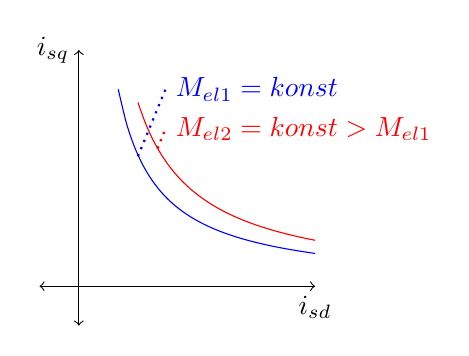
\begin{tikzpicture}[scale=0.5]
%koordinatni sistem
\draw [<->](-1,0)--(6,0) node[anchor=north]{$i_{sd}$};
\draw [<->](0,-1)--(0,6) node[anchor=east]{$i_{sq}$};

\draw[scale=1,domain=1:6,smooth,variable=\x,blue] plot ({\x},{5/\x});

\draw[dotted,blue,thick](1.5,3.3)--(2.2,5) node[anchor=west]{$M_{el1}=konst$};
\draw[dotted,red,thick](2,3.5)--(2.2,4) node[anchor=west]{$M_{el2}=konst >M_{el1}$};
\draw[scale=1,domain=1.5:6,smooth,variable=\x,red] plot ({\x},{7/\x});

\end{tikzpicture}
\caption{Prikaz navora v odvistnosti od komponent toka }
\label{fig:navor}
\end{figure}

Ob upo"stevanju absolutne vrednosti toka $\hat{I}~=~\sqrt{i_{sd}^2+i_{sq}^2}$, lahko hitro sklepamo, da bo navor pri konstanti amplitudi toka najvi"sji, ko sta komponenti $i_{sd}$ in $i_{sq}$ enaki.

\section{Standardna metoda}
\label{sec:stand}
Napajalni pretvornik pogona ima definirano napetostno in tokovno limito. Napetostna limita je odvisna od napetosti enosmernega pretvornika.\cite{vas}
Zaradi omejene izhodne napetosti pretvornika je lahko maksimalna napetost:
\begin{equation}
u_{sd}^2+u_{sq}^2= U_{smax}^2
\label{eq:napetostna_limita_osnovna}
\end{equation}

$u_{sd}$ in $u_{sq}$ predstavljata vzdol"zno in pre"cno komponento  napetosti v dvoosnem koordinatnem sistemu. Napetosti sta odvisni od pre"cne $i_{sq}$ in vzdol"zne $i_{sd}$ komponente toka ter magnetilnega  toka $i_{mr}$ (ena"cbi \ref{eq:usd}, \ref{eq:usq}). Magnetilna komponenta toka je odvisna le od $i_{sd}$ (\ref{eq:imr}). Magnetilna komponenta se na $i_{sd}$ odziva, kot "clen prvega reda s "casovno rotorsko konstanto ki je razmerje  med rotorsko induktivnostjo in rotorsko upornostjo.\cite{servopogoni}

\begin{equation}
u_{sd}= R_s i_{sd}+L_s' \frac{di_{sd}}{dt}- L_s' \omega_{mr} i_{sq}+(L_s-L_s')\frac{di_{mr}}{dt}
\label{eq:usd}
\end{equation}
\begin{equation}
u_{sq}= R_s i_{sq}+L_s' \frac{di_{sq}}{dt} + L_s' \omega_{mr}i_{sd}+(L_s-L_s')\omega_{mr}i_{mr}
\label{eq:usq}
\end{equation}

\begin{equation}
T_r\frac{di_{mr}}{dt}+i_{mr} =i_{sd}
\label{eq:imr}
\end{equation}
\begin{equation}
T_r=\frac{L_r}{R_r}
\label{eq:Tr}
\end{equation}


V stacionarnem stanju so vrednosti odvodov enake 0. Magnetilni tok ima takrat enako vrednost kot $i_{sd}$. Pri vi"sjih vrtilnih hitrostih postane ohmski padec napetosti zanemarljiv in ena"cbi se v stacionarnem stanju poenostavita v

\begin{equation}
u_{sd}= - L_s' \omega_{mr} i_{sq}
\label{eq:usd_stat_w}
\end{equation}
\begin{equation}
u_{sq}=  L_s \omega_{mr}i_{sd}
\label{eq:usq_stat_w}
\end{equation}
 Vstavimo (\ref{eq:usd_stat_w}) in (\ref{eq:usq_stat_w}) v ena"cbo (\ref{eq:napetostna_limita_osnovna})

\begin{equation}
(L_s' \omega_{mr} i_{sq})^2+(L_s \omega_{mr}i_{sd})^2= U_{smax}^2
\label{eq:napetostnalim1}
\end{equation}

Rezultat predstavlja maksimalno vrednost statorskih tokov v dvoosnem koordinatnem sistemu, v odvisnosti od napetosti. "Ce izraz nekoliko predelamo dobimo ena"cbo, iz katere prepoznamo elipso: 

\begin{equation}
(\frac{i_{sd}}{a})^2+(\frac{i_{sq}}{b})^2 = 1
\label{eq:napetostnalim}
\end{equation}

$a$ in $b$ predstavljata pol osi elipse, $a=U_{smax}/(\omega_{mr}L_s)$, $b=U_{smax}/(\omega_{mr}L_s')$. Polosi sta funkciji vrtilne hitrosti in z nara"s"canjem hitrosti postajati manj"si.

Vsak motor je konstruiran za dolo"cene pogoje in temu primerno je dolo"cen tudi nazivni tok. "Ce stroj obratuje z vi"sjim tokom kot je nazivni, se bo zaradi toplotnih izgub v navitjih za"cel segrevati. S segrevanjem se lahko stroj deformira, ali se mu z obratovanjem v takih pogojih skraj"sa "zivljenska doba. Maksimalen tok v motor je tako definiran kot:

\begin{equation}
i_{sd}^2+i_{sq}^2=\hat{I}_{n}^2=I_{smax}^2
\label{eq:tokovnalim}
\end{equation}

Pogojema dolo"cenima z ena"cbama (\ref{eq:napetostnalim}) in (\ref{eq:tokovnalim}), mora statorski tok vedno ustrezati. Ob takem obratovanju bo stroj lahko deloval celotno "zivljensko dobo.\cite{vas}

"Ce grafi"cno ponazorimo napetostno in tokovno limito nam presek limit prikazuje to"cko, ki ozna"cuje najve"cjo vrednost $i_{sd}$ in $i_{sq}$ (Slika \ref{fig:napetostna_tokovna_limita_slika}). V tej to"cki motor ustvari najve"cji navor. Tokovna limita je ponazorjena s kro"znico, z radijem $I_{smax}$. Elipsa predstavlja napetostno limito, ki se v odvisnosti od vrtilne hitrosti spreminja. Pri ni"zjih vrtilnih hitrostih sta polosi ve"cji od polmera tokovne limite (Napetostna limita za $\omega_1$ na sliki \ref{fig:napetostna_tokovna_limita_slika}), zato vpliva na "zeljene vrednosti tokov $i_{sd}$ in $i_{sq}$ le tokovna limita (tokovni vektor se mora gibati znotraj zelenega kroga). Pri vi"sjih vrtilnih hitrostih polosi elipse postaneti manj"si in "zelene vrednosti tokov se morajo prilagoditi tudi napetostni limiti (Napetostna limita za $\omega_2$ na sliki \ref{fig:napetostna_tokovna_limita_slika}). "Zeleni vrednosti tokov $i_{sd}$ in $i_{sq}$ se morati prilagoditi preseku obmo"cja, ki ga ozna"cuje obarvan del. 

\begin{figure}
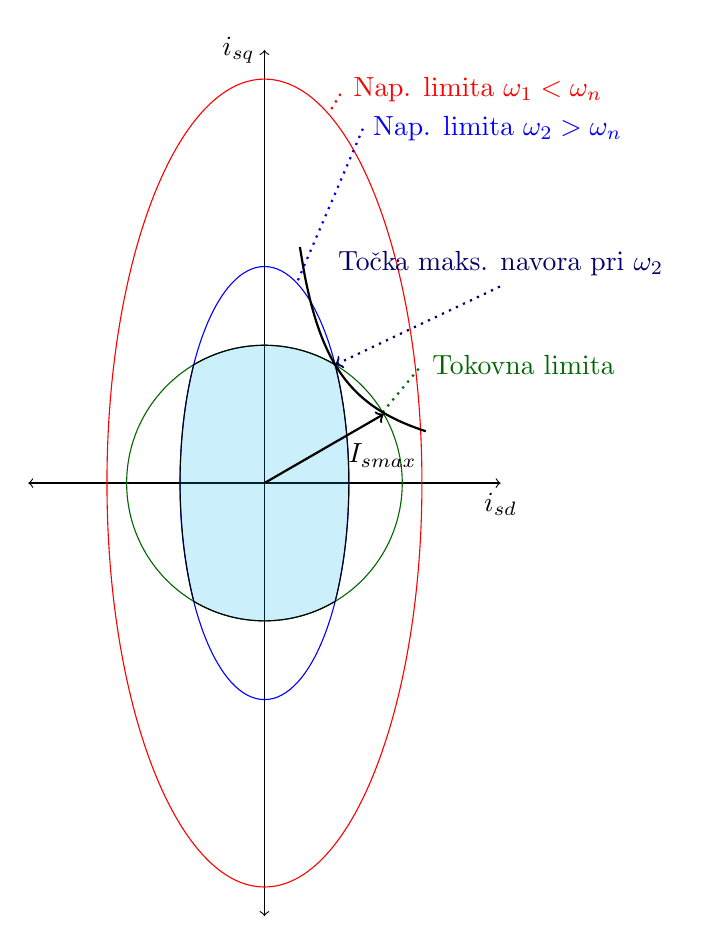
\begin{tikzpicture}[scale=0.5]
%koordinatni sistem
\draw [<->](-6,0)--(6,0) node[anchor=north]{$i_{sd}$};
\draw [<->](0,-11)--(0,11) node[anchor=east]{$i_{sq}$};

%elipsa za nizke hitrosti
\draw [red](0,0)ellipse  (4 and 10.26);
\draw [dotted,red,thick] (1.7,9.5)--(2,10) node[anchor=west]{Nap. limita $\omega_1 < \omega_n $};

%elipsa za visoke hitrosti
\draw [dotted,blue,thick] (0.85,5.15)--(2.5,9) node[anchor= west]{Nap. limita $\omega_2 > \omega_n$};
\draw [blue] (0,0)ellipse (2.145 and 5.5);

%tokovna limita in oznacba
\draw [black!60!green](0,0)circle (3.5); 
\draw [dotted,black!60!green,thick] (3,1.8)--(4,3) node[anchor= west]{Tokovna limita};

    \fill[cyan,draw=black, fill opacity=0.2] (1.79693,-3.0035) arc (-33:33.1:2.145 and 5.5)--(1.79693,3.0035)arc(59.1:180-59.1:3.5)--(-1.79693,3.0035) arc (180-33:180+33:2.145 and 5.5)--(-1.79693,-3.0035)arc(180+59.1:360-59.1:3.5);
    \draw [<-,dotted,black!60!blue,thick] (1.79693,3.0035)--(6,5) node[anchor= south]{To"cka maks. navora pri $\omega_2$};
    
\draw[->, thick](0,0)--(3.03,1.75);
\draw (3,0.7) node{$I_{smax}$};
\draw[scale=1,domain=0.9:4.1,smooth,variable=\x,black,thick] plot ({\x},{5.397/\x});

\end{tikzpicture}
\caption{Prikaz napetostne in tokovne limite pri dveh razli"cnih vrtilnih hirostih}
\label{fig:napetostna_tokovna_limita_slika}
\end{figure}

Pri vrtilnih hitrostih vi"sjih od nazivne se standardno uporablja slabljenje polja po prvi potenci. Pri tej metodi se zni"zuje vrednost toka $i_{sd}$ v obratnem razmerju z vrtilno hitrostjo,
\begin{equation}
\label{eq:standardna_metoda}
i_{sd}^*=i_{sdn}\frac{\omega_n}{\omega_r}
\end{equation}

kjer $i_{sdn}$ predstavlja nazivno vrednost magnetilnega toka, $\omega_{n}$ predstavlja nazivno vrtilno hitrost, ki jo ponvadi navede proizvajalec in $\omega_{r}$ trenutno vrtilno hitrost rotorja. Ulomek $\frac{\omega_r}{\omega_n}$ bi lahko nadomestili tudi z vrtilno hitrostjo v p.u. sistemu. Maksimalna vrednost $i_{sq}$ pri tej metodi dolo"ci limita po (\ref{eq:tokovnalim}).\cite{vas}

\begin{equation}
i_{sqmax}=\sqrt{I_{smax}^2-i_{sd}^{*2}}
\label{maxqtok}
\end{equation}.










\section{Izbolj"sana metoda}

Za zagotovitev maksimalnega navor v obmo"cju nad nazivno hitrostjo, mora biti maksimalen produkt tokov $i_{sd}$ in $i_{sq}$. Maksimalen produkt je v to"cki preseka tokovne in napetostne limite na sliki \ref{fig:napetostna_tokovna_limita_slika}.

V nadeljevanju sta opisani dve tehniki nastavljanja "zelene vrednosti vzdol"znega toka, s katerima je mo"zno dose"ci vi"sji navor kot s standardno metodo. Predpostavljamo linearno karakteristiko magnetilne krivulje $B(H)$, katera je v realnosti nelinearna. Prva tehnika (Tehnika A) ustvari ve"cji navor v obmo"cju nad vrtilno hitrostjo kot standardna. Druga (Tehnika B) temelji na prvi metodi, vendar lahko ob prehodnih pojavih ustvari ve"cji navor kot tehnika A.\cite{vas}

\subsection{Tehnika A}
\label{sec:prva_metoda}


Ob definiranem napajalnem pretvorniku je podana makismalno vrednost izhodne napetosti in toka. Ob upo"stevanju ena"cb (\ref{eq:napetostnalim}) in (\ref{maxqtok}) lahko izrazimo vrtilno hitrost, pri kateri je nazivni vzdol"zni tok "se mo"zen. Vrtilna hitrost, pri kateri se poslu"zimo tehnike slabljenja polja, je odvisna od parametrov napajalnega pretvornika, nazivnega vzdol"znega toka ter statorske in stresane induktivnosti. 

\begin{equation}
\omega_n=\frac{{U}_{smax}}{\sqrt{i_{sdn}^{2}(L_s^2-L_s'^2)+(L_s'I_{smax})^2}}
\label{nazivnaw}
\end{equation}



V podro"cju slabljenja polja bo navor vi"sji od standardne metode ob upo"stevanju limit, ki jih dolo"cati ena"cbi (\ref{eq:napetostnalim}) in (\ref{eq:tokovnalim}). 

\begin{equation}
\label{eq:zeljentok1}
i_{sd}^*=\sqrt{\frac{(\frac{U_{smax}}{\omega})^2-(L_s'I_{smax})^2}{L_s^2-L_s'^2}}
\end{equation}

Vrednost $i_{sd}^*$ glede na vrtilno hitrost v podro"cju slabljenja polja lahko razberemo iz slike \ref{fig:napetostna_tokovna_limita_slika}, v prese"ci"s"cu elipse in kro"znice. 

Za zagotovitev "cim vi"sjega navora in najoptimalnej"sih statorskih tokov v nadnazivnih hitrostih, je potrebno upo"stevati ena"cbo za limito napetosti (\ref{eq:napetostnalim1}) in navorne ena"cbe (\ref{eq:navor1}). Iz (\ref{eq:napetostnalim1}) izrazimo eno od komponent toka, jo vstavimo v (\ref{eq:navor1}), odvajamo po drugi komponenti toka in ena"cimo z ni"c. Iz postopka sledi, najoptimalnej"se obratovanje pri tokih

\begin{equation}
\label{eq:optimum_d}
i_{sd}=\frac{U_{smax}}{\omega \sqrt{2}L_s}
\end{equation} 
\begin{equation}
\label{eq:optimum_q}
i_{sq}=\frac{U_{smax}}{\omega \sqrt{2}L_s'}
\end{equation} 
Z vstavljanjem v (\ref{eq:napetostnalim1}) opazimo, da je najoptimalneje obratovati z enakima komponentama napetosti $u_{sd}$ in $u_{sq}$.\cite{vas}

\subsection{Tehnika B}
\label{sec:druga_metoda}

Pri tehniki A je upo"stevano, da je motor v stacionarnem stanju in mangetilni tok enak $i_{sd}$.
Navorno ena"cbo za asinhroski motor se lahko zapi"se kot:\cite{servopogoni}
\begin{equation}
\label{eq:navor2}
M_{el}=\frac{3}{2}p_p \frac{L_m}{L_r}|\psi_{rd}|i_{sq}
\end{equation}
Pri "cemer $\psi_{r}$ predstavlja rotorski magnetni sklep. Ta je odvisen od magnetilnega toka, ki je posledica $i_{sd}$
\begin{equation}
\label{eq:flux}
\psi_{rd}= \frac{L_m i_{sd}}{1+T_r p},
\end{equation}
kjer $p$ predstavlja operator odvajanja po "casu $p=d/dt$ in $T_r$ rotorsko "casovno konstanto.

Re"sitev ena"cebe (\ref{eq:flux}) je:
\begin{equation}
\label{eq:Lm+delta}
\psi_{rd}=L_m i_{sd}+\Delta \psi_{rd}\mathrm{,}
\end{equation}
 kjer je
 
 \begin{equation}
\label{eq:delta}
\Delta \psi_{rd}=(\psi_{rd}(t_0)-L_m i_{Sd}(t_0))e^{\frac{t_0-t}{T_r}}
\end{equation}
$t_0$ predstavlja za"cetni "cas. Elektromagnetni navor je tako povi"san
\begin{equation}
\label{navor3}
M_{el}=\frac{3}{2}p_p \frac{L_m}{L_r}(L_m i_{sd}+\Delta \psi_{rd})i_{sq}
\end{equation}

Ob upo"stevanju neenakosti magnetilnega toka in vzdol"zne komponente statroskega toka v ena"cbi \ref{eq:usq} in posledi"cno tudi v ena"cbi \ref{eq:napetostnalim}, je "zeljena vrednost vzdol"zne komponente toka:
\begin{equation}
\label{eq:zeljentok2}
\centering
\begin{multlined}
i_{sd}^*= \\ \\
\frac{\sqrt{(c L_s)^2+d[(\frac{U_{smax}}{\omega})^2-L_s'^2I_{smax}^2-c^2]}-cL_s}{d}                 
\end{multlined}
\end{equation}
\begin{equation}
i_{sqmax}=\sqrt{I_{smax}^2-i_{sd}^{*2}}
\end{equation}
Pri "cemer
$$c=\frac{L_m}{L_r}(\psi_{r}(t_0)-L_m i_{sd}(t_0))$$
$$d=L_s^2-L_s'^2$$
Po prehodnem pojavu (Ena"cba (\ref{eq:flux})), $c$ konvergira k 0. S tem se izraz (\ref{eq:zeljentok2}) poenostavi v (\ref{eq:zeljentok1}).\cite{vas}

\section{Simulacije in uporaba tehnik}
Simulacije sem izvedel s programskim paketom Matlab. 
Za model asinhronskega motorja sem si izbral naslednje podatke:
\begin{table}
\centering
\label{tab:nazivni_podatki_motorja}
\caption{Nazivni podatki simuliranega motorja}
\begin{tabular}{|c|c|}
\hline
	$P_n$		&0.5 kW \\\hline
	$M_n$		&2,5 Nm \\\hline
	$U_n$		&	15 V\\\hline
	$I_{mrn}= i_{sdn}$&	18,7 A\\\hline
	$I_n $		&	28,4 A\\\hline
	$n_N $		&	2200 rpm\\\hline
	$R_s$		&	0.074 $\mathrm{\Omega}$\\\hline
	$R_r$		&	0.0513 $\mathrm{\Omega}$\\\hline
	$L_s $		&	2.596 mH\\\hline
	$L_r $		&	2.559 mH\\\hline
	$L_m $		&	2.4 mH\\\hline
	$p_p $		& 	1 polov par	\\\hline
	$J$			&	0,001 kg $\mathrm{m}^2$	\\\hline										
\end{tabular}
\end{table}



Za izra"cune v simulaciji sem uporabil dvoosni koordinatni sistem, v katerega sem pretvoril asinhronski motor.

%Simuliran napetostni pretvornik je imel omejitve napetosti in toka prilagojene nazivnim parametrom asinhronskega motorja.
%\begin{itemize}
%\item{$U_{dc}=U_{max}=U_n\sqrt{2}=21,2$ V}
%\item{$I_{max}=I_n\sqrt{2}=40,16$ A}
%\end{itemize}



Motor sem reguliral z neposredno FOC metodo. Limite v regulaciji sem nastavil po izrazih v \ref{eq:napetostnalim1} in \ref{eq:tokovnalim}.
Osrednji del simulacij se je navezoval na dolo"canje vzdol"zne komponente toka. Za njeno dolo"canje sem uporabil izraza iz zgoraj teoreti"cno opisanih postopkov (Glej poglavje \ref{sec:prva_metoda}, \ref{sec:druga_metoda}).

\section{Rezultati simuliranih tehnik}

Pri simulaciji izbolj"sanih tehnik nisem upo"steval nelinearnosti "zeleza. Zato je vrtilna hitrost lahko nara"s"cala tudi v obmo"cju, kjer se je v realnosti potrebno poslu"ziti druge tehnike zaradi nasi"cenosti "zeleza.

\subsection{Stati"cna karakteristika}

Stati"cno karakteristiko sem simuliral tako, da sem "zeljeno vrednost vrtilne hitrosti linearno ve"cal. Rezultat simulacije je na sliki \ref{fig:static}.

\begin{figure}
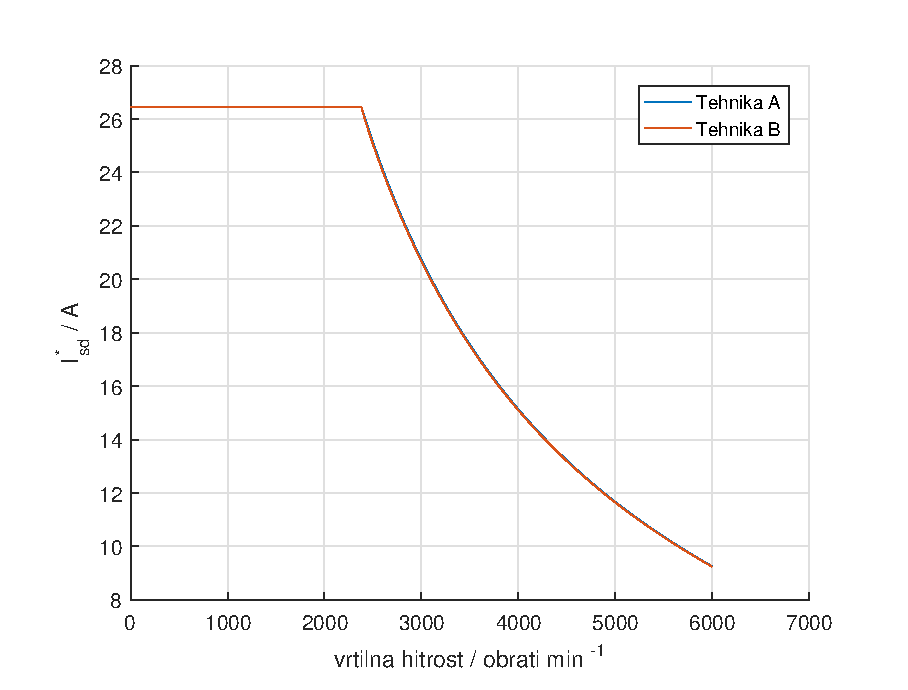
\includegraphics[width=0.55\textwidth]{fig_static.eps}
\label{fig:static}
\caption{Odvisnost "zeljene vrednosti vzdol"zne komponente toka od vrtilne hitrosti}
\end{figure}

V poglavju \ref{sec:druga_metoda} je opisano, da je v stacionarnem stanju vrednost $i_{sd}^*$ enaka v obeh tehnikah. V simulaciji je manj"se odstopanje druge tehnike. Vrednost vrtilne hitrosti sem linearno vi"sal, zato se je spreminjala tudi "zeljena vrednost vzdo"zne komponente. Rotorski magnetni pretok  linearno sledi vrednosti $i_{sd}$. Konstanta $c$ tako ni 0. Izraz v \ref{eq:zeljentok2} zato ni enak \ref{eq:zeljentok1} in od tu je manj"se odstopanje.

\subsection{Prehodni pojav}

V naslednji simulaciji sem simuliral prehode vrtilne hitrosti. Za "zeljeno vrednost vrtilne hitrosti sem nastavljal stopni"casto funkcijo. Ob tem sem opazoval vrtilno hirost, vrednosti magnetilnega toka in potek ustvarjenega navora. Dolo"canje "zeljene vrednosti $i_{sd}$ sem nastavljal z uporabo tehnik opisanih v poglavju \ref{sec:prva_metoda} in \ref{sec:druga_metoda}.
Potek simulacije je predstavljen na slikah \ref{fig:vrtilna}, \ref{fig:imr} in \ref{fig:Mel}. V podro"cju slabljenja polja se vrednost "zeljene vrednosti vzdol"zne komponente toka manj"sa.
Pri "casu 0,6~s  sem se za"cel poslu"zevati tehnik primernih v podro"cju slabljenja polja. Motor v tem podro"cju lahko ustvari manj"si navor, kot ga je lahko ustvarjal v obmo"cju pod nazivno hitrostjo. Na sliki \ref{fig:Mel} se vidi kako motor v obmo"cju vi"sjih vrtilnih hitrosti ne ustvari ve"c polnega navora. Najvi"sja vrednost ustvarjenega navora pada obratno sorazmerno z vi"sanjem vrtilne hitrosti. Prehodni pojav vrtilne hitrosti zaradi manj"sega ustvarjenega navora traja dlje (Slika \ref{fig:vrtilna}).

\begin{figure}
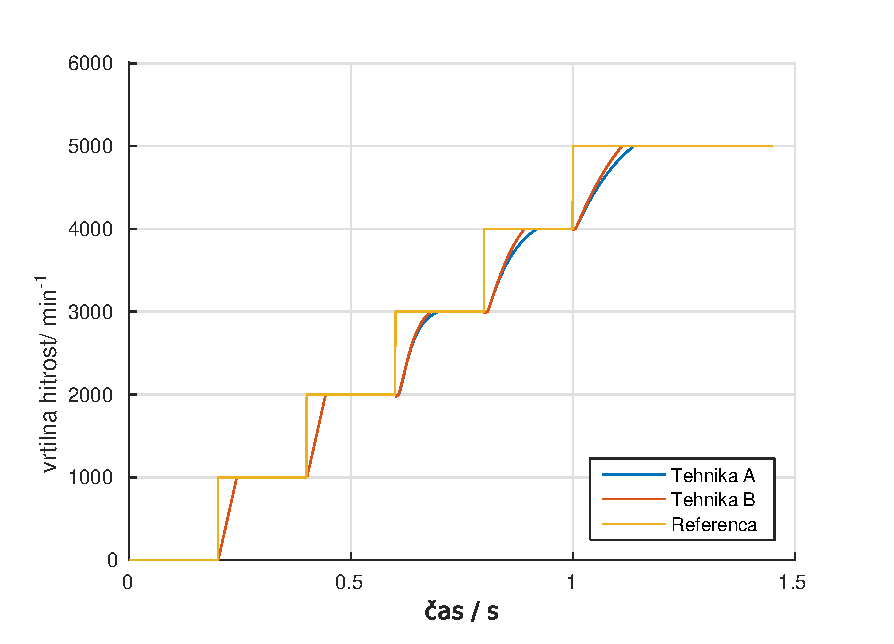
\includegraphics[width=0.55\textwidth]{fig_vrtilna.eps}
\caption{Potek prehodov vrtilne hitrosti}
\label{fig:vrtilna}
\end{figure}

\begin{figure}
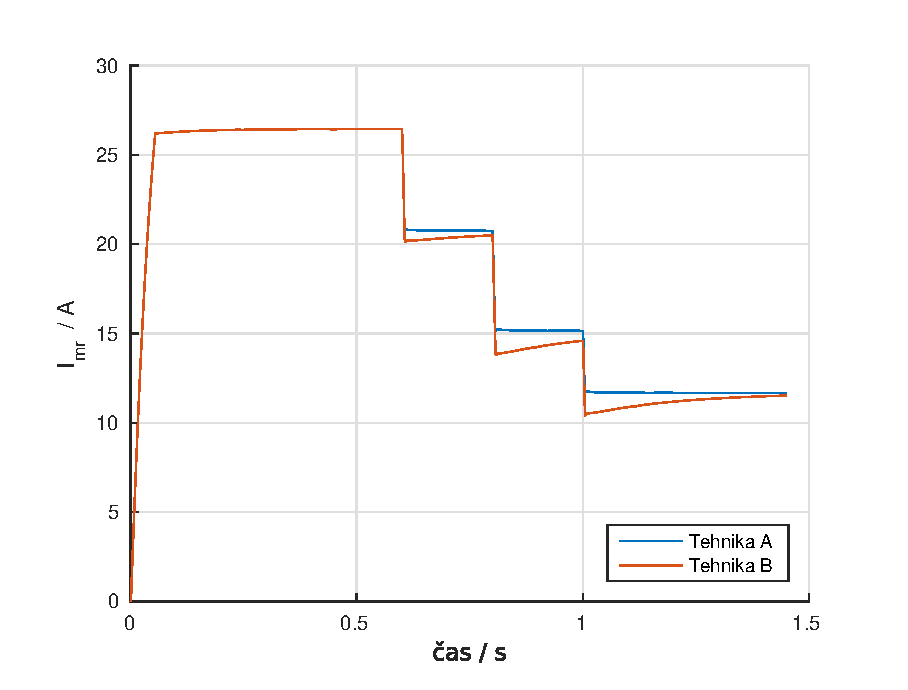
\includegraphics[width=0.55\textwidth]{fig_imr.eps}
\caption{Potek vrednosti magnetilnega toka}
\label{fig:imr}
\end{figure}



\begin{figure}
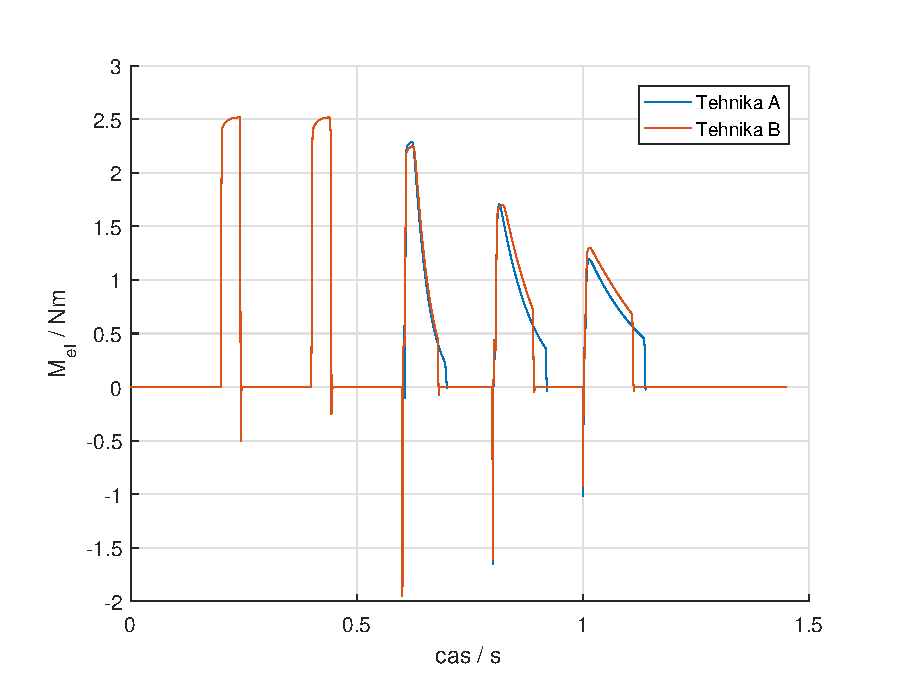
\includegraphics[width=0.55\textwidth]{fig_Mel.eps}
\caption{Potek ustvarjenega navora}
\label{fig:Mel}
\end{figure}

\section{Druge metode maksimalnega navora na tok}

V regulaciji se nastavlja vrednosti "zeljenih tokov, vendar motor se krmili z napetostjo. Izhod regulacije je napetost, katero je potrebno prilagoditi glede na  podro"cje delovanja. V podro"cju konstantnega navora je "zelja zagotoviti naziven magnetni pretok ($i_{sd}^*=$~konst.).
Izhodna napetost ima ni"zjo amplitudo kot jo lahko zagotovi enosmerni tokokrog. V tem podro"cju se uporablja U/f metoda. \cite{servopogoni} Ko U/f metoda dose"ze maksimalno izhodno napetost je potrebno pre"cno komponento napetosti manj"sati (\ref{eq:usq_stat_w}). Za ohranjanje maksimalne napetosti lahko vzdol"zno komponento napetosti povi"samo. V obratovanju z maksimalno izhodno napetostjo, se bo lahko zagotovil najvi"sji navor. Slika \ref{fig:MTPA_strategy} prikazuje primer blokovne sheme za zagotavljanje maksimalnega navora. Strategija je sestavljena iz dveh PI regulatorjev za dolo"canje vzdol"zne komponente toka in maksimalne vrednosti $i_{sq}$.

\begin{figure}
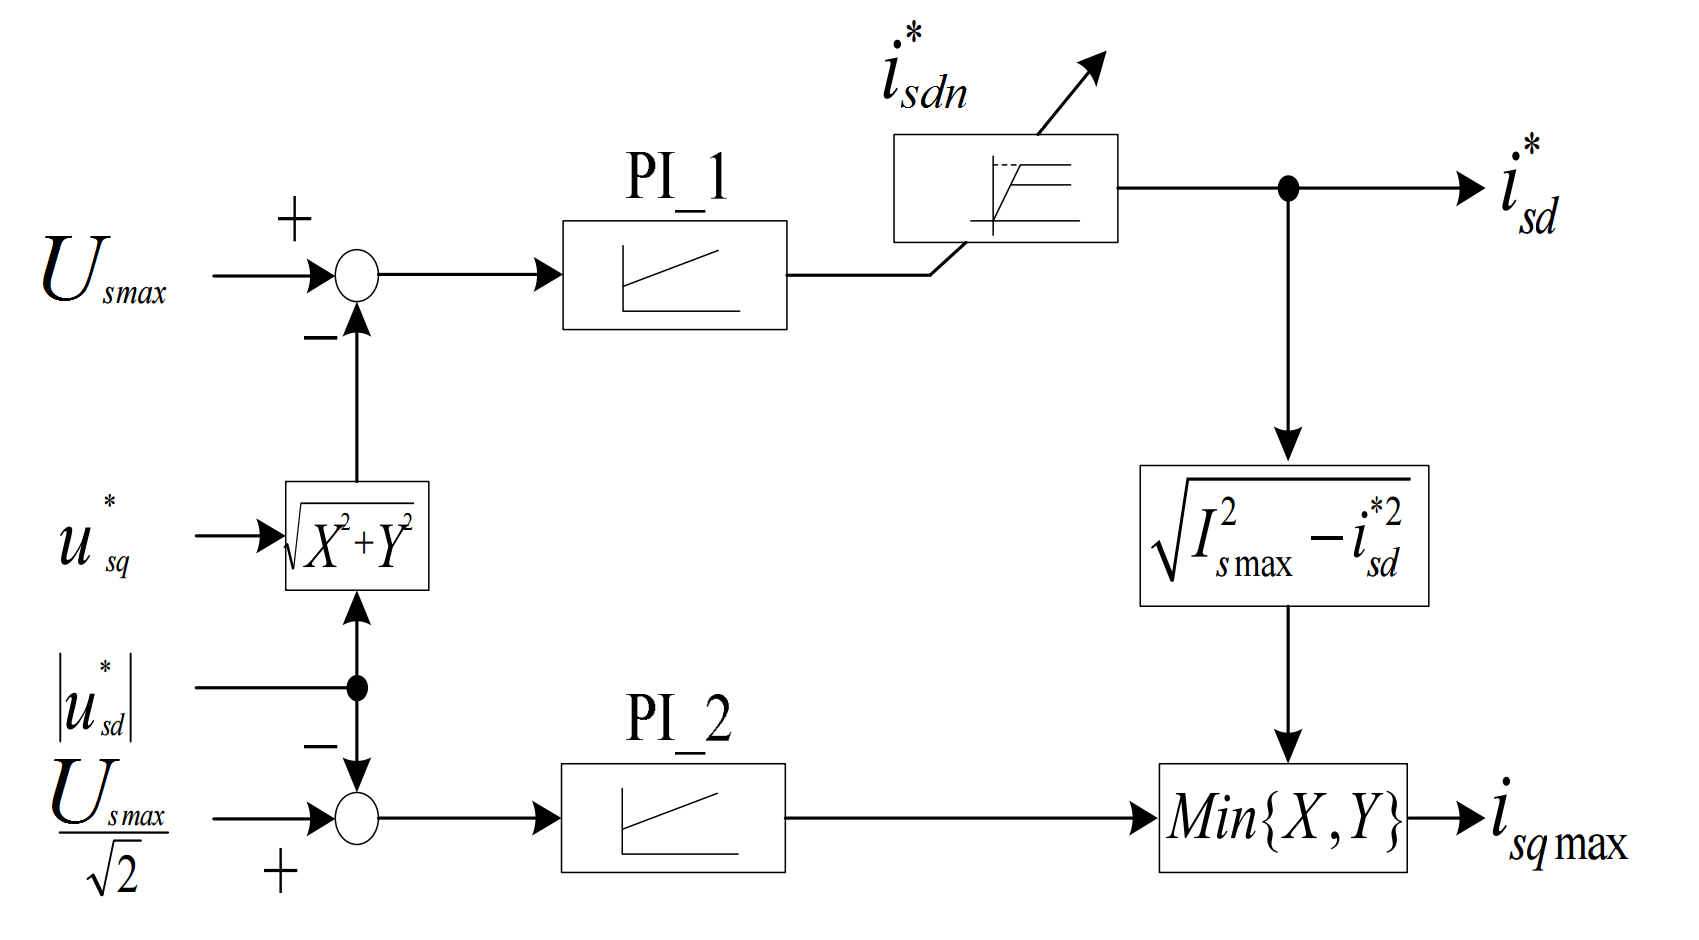
\includegraphics[width=0.5\textwidth]{MTPA_prva.png}
\caption{Blokovna shema za dolo"canje vzol"zne komponente toka in maksimalne vrednosti pre"cne komponente toka\cite{MTPA}}
\label{fig:MTPA_strategy}
\end{figure}

Regulator PI\_1 regulira vzdol"zno komponento toka in skrbi za zmanj"sevanje magnetnega pretoka v podro"cju slabljenja polja. Regulator PI\_2 skrbi, da sta vrednosti $|u_{sd}^*|$ in $u_{sq}^*$ enaki $\frac{U_{smax}}{\sqrt{2}}$ (\ref{eq:optimum_d}) (\ref{eq:optimum_q}), saj motor v tej delovni to"cki ustvari najve"cji navor(glej pog. \ref{sec:prva_metoda}).

Na sliki \ref{fig:MTPA_app} je prikazan primer uporabe takega na"cina dolo"canja "zeljenih vrednosti tokov. Regulator PI\_1 je omejen z nazivno vrednostjo vzdo"zne komponente toka in uravnava vrednost toka, ko je na izhodu zahtevana maksimalna napetost. Regulator PI\_2 je v nasi"cenju ko motor obratuje v obmo"cju konstantnega navora. Maksimalna vrednost $i_{sq}$ je omejena z izrazom $\sqrt{I_{smax}^2-i_{sd}^2}$. V tem obmo"cju je maksimalna vrednost pre"cne komponente toka odvisna le od $i_{sd}$. V podro"cju slabljenja polja se za"cne "zeljena vrednost vzdol"zne komponente toka manj"sati, s tem pa se za"cne vi"sati vrednost maksimalne vrednosti pre"cne komponente. Izhod regulatorja PI\_1 se zaradi nara"s"canja absolutne vrednosti pre"cne komponente napetosti manj"sati. So"casno za"cne regulator PI\_2 siliti kon"cno izhodno napetost vzdol"zne komponente k vrednosti $U_{smax}/\sqrt{2}$. Rezultat delovanja s to strategijo je, da motor ves "cas deluje v to"cki maksimalnega navora.~\cite{MTPA}



\begin{figure}
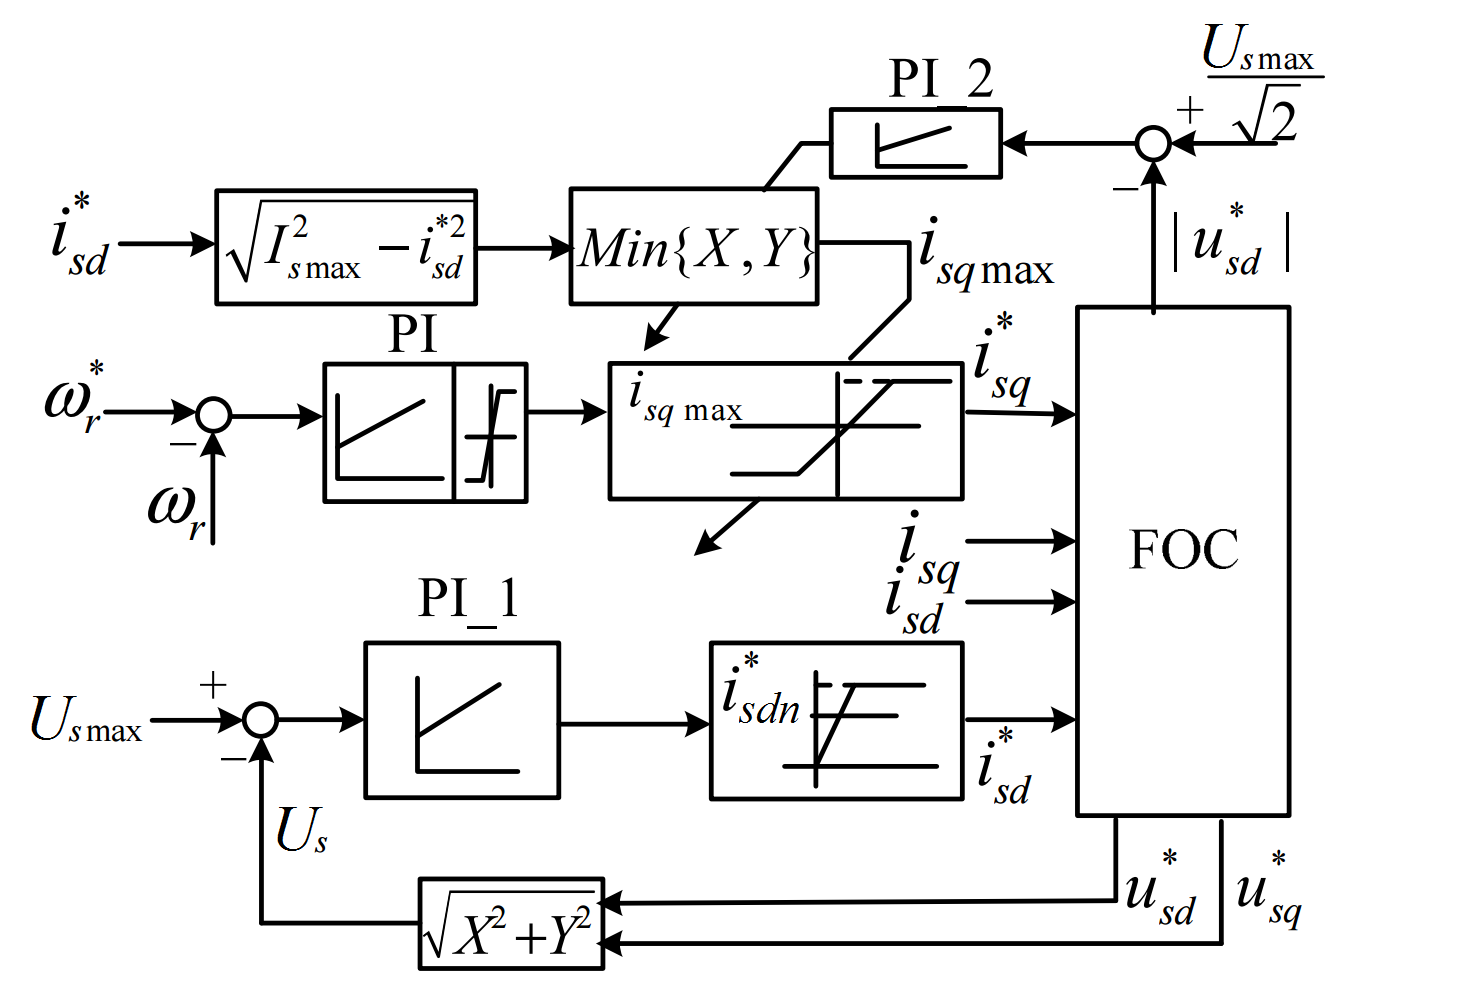
\includegraphics[width=0.55\textwidth]{MTPA.png}

\caption{Blokovna shema regulacije za ustvarjanje maksimalnega navora \cite{MTPA}}
\label{fig:MTPA_app}
\end{figure}

V opisu te regulacije nikjer ni omenjen noben parameter stroja katerega reguliramo. Metoda samodejno zni"za vrednost $i_{sd}$, ko je na izhodu maksimalana napetost. Maksimalno vrednost pre"cne komponente toka dolo"ci tokovna limita (\ref{eq:tokovnalim}), ali regulator PI\_2 glede na vrednost vzdol"zne komponente napetosti (\ref{eq:optimum_q}).To je prednost te metode, da je univerzalna za katerikoli asinhronski stroj.



\section{Zaklju"cek}

Predstavil sem regulacijo motorja v podro"cju slabljenja polja. Opisal sem osnovno metodo, kako nastavljati "zeljeno vrednost vzdol"zne komponente toka. Predstavil sem tudi izbolj"sani tehniki, s katerima lahko motor ustvari vi"sji navor v obmo"cju nad nazivno hitrostjo. Simuliral sem poteke nastavljanje vzdol"zne komponente toka glede na "zeljeno vrtilno hitrost. Na koncu sem predstavil "se metodo, katera napaja motor tako, da vedno deluje v to"cki najve"cjega ustvarjenega navora.

Vrtenje motorja v nadnazivnih hitrostih nam omogo"ca ve"cji razpon "zeljene vrtilne hitrosti. Z uporabo primernih tehnik lahko v "sirokem obmo"cju vrtilne hitrosti dose"zemo maksimalen navor. S tem delom sem prikazal, da se lahko v obmo"cju nad nazivno hitrostjo obratuje dobro. S primerno metodo se da "se zvi"sati ustvarjen navor. Metodo katero se bo uporabilo v pogonu, je nato odvisno le od na"crtovalca.


%V prehodnem pojavu razlike niso velike. Izbolj"sana metoda pa se izka"ze pri ustvarjanju navora. Pri simulirani vrtilni hitrosti je lahko regulacija motorja z izbolj"sano metodo ustvarila tudi do 30\% vi"sji navor kot standardna metoda.

%
%
%\newpage
%
%
%
%Pri asinhroskih motrojih je magnetilni tok odvisen od pre"cne komponente toka(ena"cba \ref{eq:imr}). 
%Magnetni rotorski pretok je linearno odvisen od magnetilnega toka, ta pa je posledica vzdol"zne komponente statorskega toka.
%\begin{equation}
%\label{eq:flux}
%\psi_{rd}= \frac{L_m i_{Sd}}{1+T_r p}
%\end{equation}
%
%kjer $p$ predstavlja operator odvajanja po "casu $p=d/dt$ in $T_r$ rotorska "casovna konstanta. Navorno ena"cbo lahko zapi"semo tudi kot:
%\begin{equation}
%\label{eq:navor2}
%M_{el}=\frac{3}{2}p_p \frac{L_m}{L_r}|\psi_{r}|i_{Sq}
%\end{equation}
%Z upo"stevanjem, da je magnetilni tok posledica vzdol"zne komponente, ki jo reguliramo, med spremembo vrtilne hitrosti lahko upo"stevamo tudi ta parameter. "zeljeno vrednost vzdol"zne komponente toka lahko tako dolo"cimo po ena"bi iz \cite{vas}
%\begin{equation}
%\label{eq:zeljentok2}
%i_{Sd}^*=\frac{\sqrt{(c L_s)^2+(L_s^2-L_s'^2)[(\frac{U_{dc}}{\omega})^2-L_s'^2I_{smax}^2-c^2]}-cL_s}{L_s^2-L_s'^2}
%\end{equation}
%pri "cemer
%$$c=\frac{L_m^2}{L_r}(i_{mr}-i_{Sd})$$.
%V stacionarnem stanju sta magnetilni tok in vzdol"zna komponenta statorskega toka enaki in $c=0$. Izraz v  \ref{eq:zeljentok2} se poenostavi v izraz iz prve metode(ena"cba \ref{eq:zeljentok1})
%Elektromagnetni navor se lahko izrazi sedaj tudi:
%\begin{equation}
%\label{eq:navorzatok2}
%M_{el}=\frac{3}{2}p_p \frac{L_m}{L_s' L_r}\sqrt{(\frac{U_{dc}}{\omega})^2-(L_s i_{Sd}^*+c)^2\psi_{rd}}
%\end{equation}

%\begin{table}[!t]
%%\renewcommand{\arraystretch}{1.3}
%%\caption{Rezultati optimizacije D flip-flopa}
%%\label{results}
%%\centering
%%\begin{tabular}{l @{\hspace{-2mm}} r | r r r}
%%lastnost                                    &                   & original           & hitrost & poraba \\ \hline 
%%\multicolumn{4}{l}{\scriptsize $\uparrow$ in $\downarrow$ pomenita naraščajočo in padajočo fronto} \\
%%\end{tabular}
%%\end{table}
%%
%%V stolpcu poraba v tabeli \ref{results} so zbrani vadno uporabljena hitra lokalna optimizacijska metoda, npr. \cite{hooke}. Žal p
%%
%%%\centerline{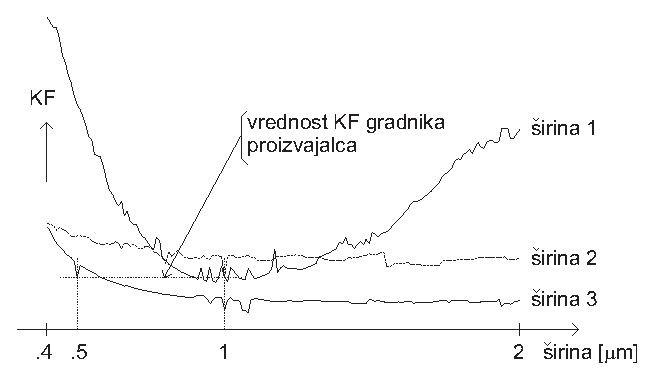
\includegraphics[width=8cm]{fig/cost_profile_slo}}



\begin{thebibliography}{10}

\bibitem[1]{servopogoni}V.~Ambro"zi"c, P.~Zajec, {\em Elektri"cni servo pogoni}, \hskip 1em plus 0.5em minus 0.4em \relax Slovensko zdru"zenje elektroenergetikov CIGR\'E-CIRED, 2016

\bibitem[2]{miljavc}P.~Jereb, D.~Miljavec, {\em Elektri"cni  stroji: temeljna znanja}, \hskip 1em plus 0.5em minus 0.4em \relax Fakulteta za elektrotehniko, Ljubljana, 2014


\bibitem[3] {denis}D.~Su"sin, {\em Transformacije}



\bibitem[4]{vas} P.~Vas, {\em Sensorless Vector and Direct Torque Control}, \hskip 1em plus 0.5em minus 0.4em \relax Oxford University Press, pp 632--641, 1998


\bibitem[5]{MTPA}Y.~Xu, C.~Shen , H.~Hui and Z.~Huang, {\em Field Weakening Strategy in a Wide Speed Range of
Induction Motors for Electric Vehicles Based on
Maximum Torque Control}\hskip 1em plus 0.5em minus 0.4em \relax Power Electronics and Application Conference and Exposition, p. 740, 2014 
\end{thebibliography}







% that's all folks
\end{document}


